\documentclass{article}

\usepackage{amsmath} % math stuff
\usepackage{amssymb} % math stuff
\usepackage{array} % equations and stuff
\usepackage{bm} % bold math
%\usepackage{booktabs} % extra table rule options
%\usepackage{caption} % suppressed table numbering; incompatible with revtex, and longtable, I think
\usepackage{comment} % comment environment
%\usepackage{enumitem} % customization of enumeration, itemize, and description
\usepackage[T1]{fontenc} % font encoding for special characters, must also use scalable font package
\usepackage[margin=0.8in]{geometry} % paper sizes and margins (but be careful not to mess up pre-defined pages)
\usepackage{graphicx} % for graphics
%\usepackage{helvet} % default font is the helvetica postscript font
\usepackage{layouts} % print units like widths
\usepackage{lipsum} % lorem ipsum filler text
\usepackage{lmodern} % scalable font?
\usepackage{longtable} % multi-page tables
\usepackage{makecell} % specify line-breaks in table cells
\usepackage{mathrsfs} % math script font
\usepackage{mhchem} % easier chemical formula
\usepackage{microtype} % allows disabling of ligatures
%\usepackage{newcent} % new century schoolbook font
\usepackage{nicefrac}
\usepackage{numprint} % print and format (large) numbers
\usepackage{parskip} % removes paragraph indentation, and adjusts paragraph skip, as well as list items
\usepackage{pdfpages} % add pdf files as pages
%\usepackage{setspace} % adjust text spacing and indents
\usepackage{siunitx} % decimal alignment
\usepackage{subfigure} % divided figures
%\usepackage{tabu} % extra table options
\usepackage{textcomp} % symbols
\usepackage{threeparttablex} % better footnotes with longtable
\usepackage{titling} % title placement
\usepackage{ulem} % strikethrough text
%\usepackage{url} % superceded by hyperref
\usepackage{verbatim} % verbatim environment
\usepackage{xcolor} % colors and color boxes
\usepackage{xspace} % commands that don't eat up white space
\usepackage{hyperref} % links and page setup; should always come last

\hypersetup{
 bookmarks=true,
 colorlinks=true,
 citecolor=blue,
 linkcolor=blue,
 urlcolor=blue,
 pdfstartview={XYZ null null 1.0} % default open view is 100%
}

\DisableLigatures[f,t]{encoding = T1} % disable ff, fi, fl, tt ligatures; without options, it also disables -- = endash
\renewcommand{\arraystretch}{1.0} % extra vertical (and horizontal?) space in tables

% define centered, left- and right-aligned columns with specified widths
\newcommand{\PreserveBackslash}[1]{\let\temp=\\#1\let\\=\temp}
\newcolumntype{C}[1]{>{\PreserveBackslash\centering}p{#1}}
\newcolumntype{L}[1]{>{\PreserveBackslash\raggedright}p{#1}}
\newcolumntype{R}[1]{>{\PreserveBackslash\raggedleft}p{#1}}

\begin{document}

\pagestyle{empty} % don't number pages

% custom title
\begin{center}
{\LARGE Classic Riddler}

\vspace{0.15in}

{\Large 16 April 2021}
\end{center}


\section*{Riddle:}

After a new moon, the crescent appears to grow slowly at first.
At some point, the moon will be one-sixth full by area, then one-quarter full, and so on.
Eventually, it becomes a half-moon, at which point its growth begins to slow down.
The animation below provides some insight into what's happening here:

\vspace{0.1in}
\begin{center}
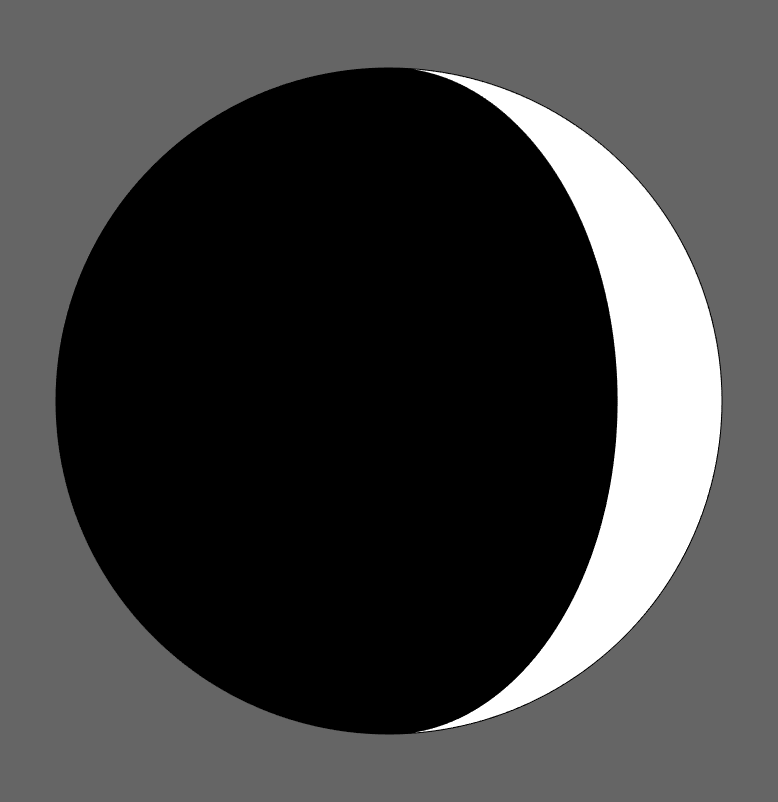
\includegraphics[width=4in]{moon_still.png}
\end{center}
\href{https://fivethirtyeight.com/wp-content/uploads/2021/04/moon_538.gif}{Link}
\vspace{0.1in}

How many times faster is the area of the illuminated moon growing when it is a half-moon versus a one-sixth moon?

(Some simplifying assumptions you might make for this problem are that the moon is a perfect sphere, that its orbit around Earth is a perfect circle, that the moon orbits the Earth much faster than the Earth orbits the sun and that the sun is very, very far away.
If you make additional assumptions, feel free to include them in your response.)


\section*{Solution:}

The moon as viewed from Earth becomes a 2-d circle, as a projection of the 3-d surface of the half-sphere that is illuminated.
The shape of the projected illumination (or it's complement) on either side (left or right) is essentially a semicircle which is compressed horizontally.
The compression depends on the angle of the rotation, which I will call $\theta$.
Basically, the area $A$ of the illuminated projection changes proportionally to $\sin\theta$, or

\[
\frac{dA}{d\theta}=k\cdot\sin\theta
\]

for some $k$.
Integrating this gives:

\[
A=-k\cdot\cos\theta+C
\]

Letting $\theta=0$ represent the new moon ($A=0$), and letting the maximum area be 1, these become

\[
\frac{dA}{d\theta}=\frac{\sin\theta}{2}
\]
\[
A=\frac{1-\cos\theta}{2}
\]

When $A=\nicefrac{1}{6}$, $\theta=\cos^{-1}(\nicefrac{2}{3})$, and $\nicefrac{dA}{d\theta}=\nicefrac{\sqrt{5}}{6}$.
When $A=\nicefrac{1}{2}$, $\theta=\nicefrac{\pi}{2}$, and $\nicefrac{dA}{d\theta}=\nicefrac{1}{2}$.
Taking the ratio of these leads to the solution of
\fcolorbox{red}{white}{$\bm{{\nicefrac{3\sqrt{5}}{5}\approx1.342}}$}\,.


\end{document}